\subsection{Penjili \& \newspeak}

\begin{frame}{Le projet Penjili}

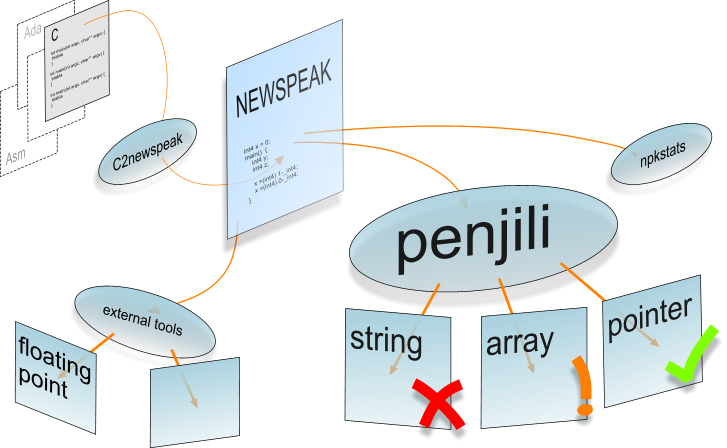
\includegraphics[scale=.5]{img/penjili.png}

\begin{tikzpicture}[remember picture, overlay]

    \node at ($ (current page.north) + (-1.5, -3.7) $) (A) {};
\only<2>{
    \node[ draw
         , shape=ellipse
         , shade
         , top color=cyan!30
         , bottom color=white
         , draw=blue!40!black!60
    ] at ($ (A) + (3, 1) $) (PT) {\texttt{ptrtype}};

    \node at ($ (PT) + (3, 0.5) $) (PTOK) {\parbox{2cm}{\centering Analyse par typage}};

    \draw[thick, orange, ->] (A) to[bend left=10] (PT);

    \draw[thick, orange, ->] (PT) to[bend left=10] (PTOK);
}
    \path (A) rectangle ++ (7cm, 2cm);

\end{tikzpicture}
\end{frame}

% TODO dire pourquoi Penjili ne convient pas
% TODO et dire ici ce que c'est que le typage

\begin{frame}{Le langage intermédiaire \newspeak}

Un langage adapté à l'analyse statique:

\begin{itemize}
\item simple: il contient peu de constructions
\item explicite: les effets de bords sont explicites
\item expressif: tout programme C peut être converti en \newspeak
\end{itemize}

\end{frame}

\begin{frame}[fragile]{Exemple}

\begin{SaveVerbatim}{compilnpk}
int32 x;
x =(int32) 0;
do {
    while (1) {
        choose {
            -->
                guard((10 > x_int32));
            -->
                guard(! (10 > x_int32));
                goto lbl1;
        }
        x =(int32) coerce[-2**31,2**31-1]
                        (x_int32 + 1);
    }
} with lbl1: {
}
\end{SaveVerbatim}

{\footnotesize
\begin{minipage}{0.3\linewidth}
\insertcode{npk-while.c}
\end{minipage}
\vrule\hspace{2pt}
\begin{minipage}{0.6\linewidth}
\BUseVerbatim{compilnpk}
\end{minipage}
}

\end{frame}
